\chapter{Analysis based on an application scenario}
\label{cha:ApplicationScenario}

This chapter discusses the techniques introduced in \autoref{sec:Techniques} in form of a small application scenario. It concludes with a comparison which mounts to the one technique which is used for the prototype in \hyperref[cha:implementation]{chapter 5}.

\begin{figure}[H]
	\centering
	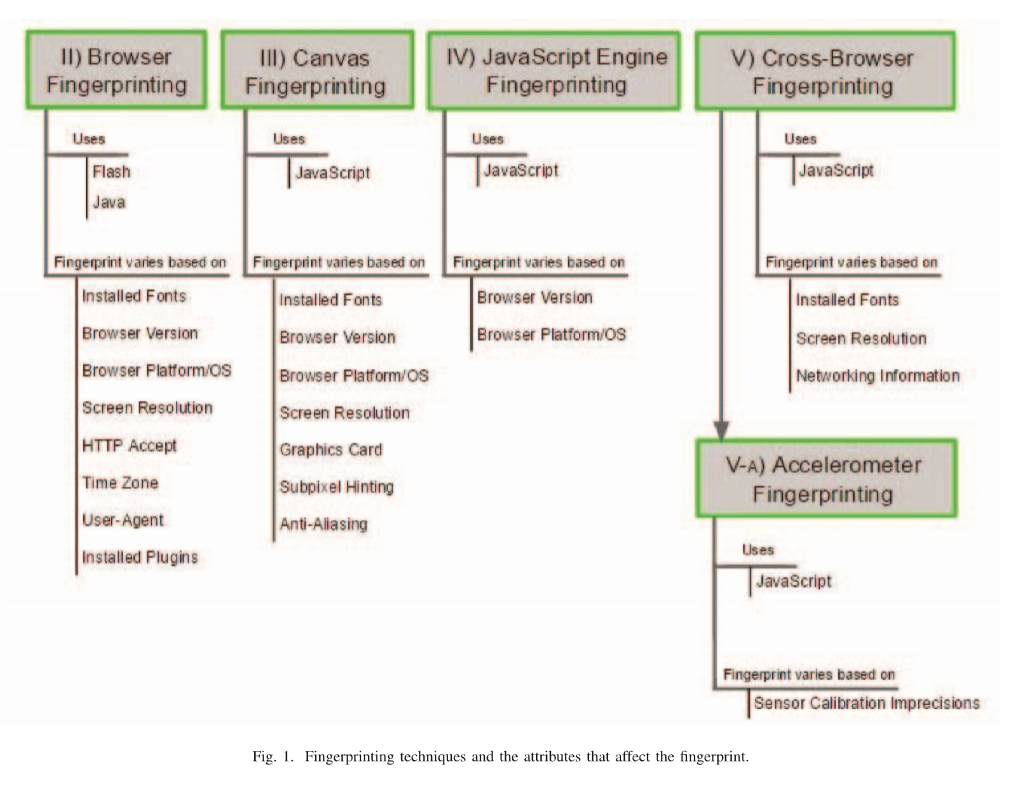
\includegraphics[width=350pt, height=160pt]{FingerprintingAttributes.png}
	\caption{Fingerprinting techniques and the attributes that effect the fingerprint}
	\label{BrowserSpecification}
\end{figure}

-- refere to previous chapter
-- give good overview what needs what?

\section{Browser specific fingerprinting}
As seen in \autoref{sec:Methods} and \autoref{specFP} browser specific fingerprinting can be an active as well as a passive fingerprinting method, depending on how the used information is acquired.


\section{Canvas fingerprinting}


\section{JavaScript Engine fingerprinting}

\section{Cross-Browser fingerprinting}

\section{Comparison}
End Comparison with and Conclusion!
As seen in the descriptions, etc.

Neither of the techniques have the ability to distinguish between multiple users on a single device.  (\textcite{upi15}, p.5)

